
\documentclass[10pt]{article} 
\usepackage[utf8]{inputenc} 
\usepackage[margin=1in]{geometry} 
\usepackage{placeins}
\geometry{a4paper} 
\usepackage{multirow}
\usepackage{graphicx}
\usepackage{amsmath}
\usepackage{multicol}
\usepackage{tikz}
\usepackage{subcaption}
\usepackage{graphicx}
\usepackage{pgfplots}
\usepackage{wrapfig}
\usepackage{amsmath,amssymb}
\usepackage{algorithmic}
\usepackage[boxruled, linesnumbered]{algorithm2e}
\usepackage{amsmath}
\newcommand\inlineeqno{\stepcounter{equation}\ (\theequation)}

\vspace{0cm}
\setlength{\parindent}{0cm}
\setlength{\parindent}{1em}
\title{ 
	Probabilistic reasoning and learning project report:  \protect\\ play Atari games using artificial neural networks \protect\\  \large a.a. 2017-2018}
\author{ Jary Pomponi}
\date{\vspace{-5ex}}

\newenvironment{Figure}
{\par\medskip\noindent\minipage{\linewidth}}
{\endminipage\par\medskip}
\newcommand{\expect}{\mathop{\mathbb{E}}\nolimits}

\begin{document}
	\maketitle
\begin{multicols}{2}
\section{Introduction}
Reinforcement learning is the area of machine learning that focuses on how agents take action in an environment in order to maximize a value called reward. Those agents should learn which action is better in each situation. In this project I have implemented different methods to teach an agent how to play Atari games just by observing the video and knowing the number of possible actions, without further information about them. In particular the game used is Pong. This approach follows the one proposed in \cite{playAtariGame} and studied deeper in \cite{playAtariGameHuman}.

\section{Q learning}

The agents act in an environment, which is formulated as a Markov decision process and defined as a tuple $(S, A, P, R, \gamma)$ in which:
\begin{itemize}
	\item $S$ is the set of possible states.
	\item $A$ is the set of possible actions.
	\item $P(s, a, s')$ is the probability of transition from state $s$ to state $s'$ taking the action $a$.
	\item $R(s, a, s')$ is the immediate reward obtained after transition from $s$ to $s'$ taking the action $a$.
	\item $\gamma$ is the discount factor (how much the future rewards are important).
\end{itemize}

At time step 0 the agent is in the initial state $s_0$ with a given probability. Then the agent pick an action $a_t$, get the reward $r_t$ and transit to the next state $s_{t+1}$. This is done until the terminal state is reached. But how the action $a_t$ should be chosen? To choose the best action in each state a function $\pi$, called policy function is used. This is a  function that specify which action to take in a given state. The optimal policy $\pi^*$ is the one that maximizes the cumulative discounted reward over time: $\sum_{t\ge0} \gamma^tr_t$.  Formally: 
\[
\pi^* = \arg \max_\pi \expect(\sum_{t\ge0} \gamma^tr_t | \pi)
\]
Following a policy produces a path in the state space. To know how good is a state a function called value function is used:
\[
V^\pi(s) =\expect(\sum_{t\ge0} \gamma^tr_t|s_0 = s,\pi )
\]
It is also possible to know how good a pair state-action is. This function is called Q function and is the one that I will mainly use:
\[
Q^\pi(s, a) =\expect(\sum_{t\ge0} \gamma^tr_t|s_0 = s, a_0 = a, \pi )
\]
 If the optimal state-action value for the next time step is known then the optimal strategy is taking the action that maximizes the expected value of $r + \gamma Q^*(s', a')$. So: 
%\[
%Q^\pi(s, a) =r+ \max_{a'} \gamma Q^* (s', a')|s, a \quad \inlineeqno
%\]
\[
Q^\pi(s, a)=\\
\]
\[ \left\{
\begin{array}{ll}
r+ \max_{a'} \gamma Q^* (s', a')|s, a & \quad	  if \: not \: terminal \\
r & \quad otherwise
\end{array}
\right. \inlineeqno
\] 
So the optimal policy can be found by iterating over all the possible pairs and computing the best action in each state, but this is not feasible if the states space is not known or if it is huge, like in the Atari case. To overcome this problem a function approximator can be used to estimate $Q(s, a)$ and $V(s)$. I will do this by using artificial neural networks.
%In this project i have used a Reinforcement learning technique called Q learning to see if an agent  

\section{Deep Q-learning (DQN)}
The basic architecture that I have used to approximate the Q function can be seen in Figure 1a. Given a state the networks calculate the expected cumulative reward for each possible action.% This improved the train performance since the Q value is calcualated The network estimates, at each step, the expected reward for each action but a mask array can be used in the train process to set to zero the unwanted action.

The problem is handled as a supervised learning one and the used loss is the so called squared error: 
\[
L(\Theta_i) = ((r + \gamma Q(s', a';\Theta_{i-i})- Q^*(s, a;\Theta_{i} ))^2
\]
Where $\Theta$ are the weights of the network. 
This is good because when a larger error shows up the network tries to minimize it, but doing this the weights change radically and with these also the target value. To overcome this problem and improve stability and convergence properties it is useful to clip rewards in -1 and 1 and to use another loss function called Huber. It takes into account the difference between large and small errors by decoupling the calculation: 
\[
 L(\Theta_i)=\left\{
 \begin{array}{ll}
 \frac{1}{2}e^2  & \quad	  if \:|e| < 1 \\
 |e| - \frac{1}{2} & \quad otherwise
 \end{array}
 \right.
\] 
where $e = r + \gamma Q(s', a';\Theta_{i-i})- Q^*(s, a;\Theta_{i} )$. This loss gives the same weight to low and high errors, improving stability and convergence.  

In the following sub-sections I will explain the used technique and architecture used in the train process. 

%A state are simply the image shown on the screen while playing and the actions are defined in the game environment. Since I work with games on a simulated tv it is preferable to skip come frames in order to speed training avoiding not useful information, since many frames will be very similar. Each state is then converted to and gray scale image and then last 4 frames are staked up and fed into the neural network. This is done because adding temporal information to the agent will result in a better action choice. 
%Moreover it should be taking into account that the networks tend to forgot past states and over-fit on current one while learning how to act. This problem is solved using a memory and a target network.
\subsection{Experience replay memory}
The approximation of Q function with an artificial neural network has a problem: while the networks learn how to act in the current state it also forgot the previous explored states. This does not allow the agent to learn how to act property. To overcome this problem the passed states are saved in a ring buffer memory with a fixed length. Those experience are random sampled each time the network is trained. A passed experience at time $t$ is saved as a tuple $(s_t, a_t, r_t, s_{t+1}, ending)$ where $ending$ indicates if the state is an ending one or not and $s_t$ are the states from $t-3$ to $t$ stacked. A subset of the memory is randomly extracted each time a network is trained. 

Fixing the length of the memory is crucial since a small one can not solve the agent's memory problem but a huge one will slow the learning process, and make this impossible in the worst case, since will contains too old states not useful in late train process.

This method can be further improved by not randomly using a probability distribution. To do that I have implemented the proportional prioritized experience replay memory presented in [CITAZIONE]. The main idea is that a transition is more desirable in the train process if the network can learn more from that. In order to know how much the network can learn from a experience it is saved in the memory with an error:
\[
error = |Q(s,a) - T(s)|
\]
Where $T(s)$ is the estimated reward obtainable from $s$. If the learning process is not started $T(s)$ is simply the immediate reward $r$. Then this error is converted to a probability $p_i= (error_i+0.001)^\beta$ where $\beta$ weight how much the higher errors are more important than others.
The sample process is the following. Each time a sample is needed a random number $s$, $0\le s \le \sum_i p_i$ is picked and the memory would be walked summing the probability of visited experience until the sum exceeds $s$, then the current transition is picked. To do that the memory should be sorted based on the $p_i$ since transitions with high error should be favorite. This is very expensive and another approach involve the used of a binary unsorted tree structure where each node contains the sum of its children. When a node is updated the change propagates through all the tree. With this structure the operation are faster and the maintenance easier. 
%Prioritized replay introduces a bias that changes the distribution uncontrollably, this can be corrected by using importance-sampling (IS) weights $w_i = (NP_i)^{-\beta}$, annealing the $\beta$ linearly to 1, that value should be reached when the train process is near to the end. Those weights are normalized by 	$1/(\max_i w_i)$ and folded into the update of the network. 

\subsection{Double DQN (target network)}
To choose the action $a$ that should be picked in a state $s$ and to estimates the future reward obtainable in the new state the same network is used. This network is like a cat chasing its own tail since the network sets itself its targets and then follow them. This could lead to instability, oscillations or divergences. This problem can be solved by using another network to estimates the future reward. 

This new network is simply a copy of the first one frozen in time, so it won't be update using a train procedure, but after several steps the weights from the first network are copied in the second one. With this improvement the Q function becomes: 
\[
Q(s, a) = r + \gamma \max_{a'} Q'(s', a') 
\]
Where $Q'$ is estimated with the second network, called target network.
A drawback is that it substantially slows down the learning process because change in the Q function is propagated only after the target network update. The intervals between updated are usually in order of thousands of steps, so this can really slow things down. But this improves the stability so it is worth to use it.

\subsection{Duel DQN (DDQN)}
Dueling DQN uses a specialized Head in order to separate Q into A (advantage) stream and a V stream. Adding this type of structure to the network head allows the network to better differentiate actions from one another, and significantly improves the learning. With this network the Q function becomes: 
\[
Q(s, a) = V(s) + (A(s, a) - \frac{1}{N} \sum_{a'}^{N} A(s, a'))
\]

The main improvement of this approach is the faster learning. In DQN the network update the Q values only for the specific actions taken in those states. This results in a slower learning as we do not learn the Q values for actions that were not taken yet. Dueling architecture starts learning the state-value even if only a single action has been taken in current state by decoupling the Q function. This architecture are shown in Figure 1b. 

\section{Training process}

As environment I have used the ai gym library with some preprocessing. The first one consist in transform the images into gray scale and resize them to $84\times84$. Then should be take into account that the Atari game are designed for TVs, so the update frequency are high and this could lead the experience memory to store too many similar images. To overcome this problem only the 4th image are taken, skipping the three before it. in addition to that a state is a stack of the last previously three not skipped states and the current one, giving the agent an overview of what happened before and help it in taking the right decision. This helps the agent to know, for example, where the ball is moving.

The agent cannot starts to learn how to move in a state space that is unknown. So it is important to explore the state space, even if it is huge, before start to learn how to act in it, otherwise the agent will move randomly since it does not know how the game is structured. To do that I have implemented the following approaches, all used at the same time:

\begin{enumerate}
\item Populate replay memory: the train process starts only when the memory contains a certain amount of experiences. This help the agent in knowing how the state space is structured before starts acting.

\item No actions taken: at the beginning of the game the agent stay stationary for a random amount of frames from 1 to 30. Those frames are not added to the memory. This helps exploration and train speed, since the starting states are all very similar. 

\item Random action pick: the probability of picking a random action in a state starts from a $\epsilon$ value and decrease linearly until a minimum is reached. This is the crucial exploration strategy since allow the agent to explore a large amount of states and associated actions while collecting the rewards. This is crucial since the agent need to know which are the useful action in the states.
\end{enumerate}
The final algorithm is: 

\begin{algorithm}[H]
\caption{Q-DQN generic algorithm}
\begin{algorithmic} 
\STATE -Initialize memory M to capacity N
\STATE -Initialize action-value function with random weights
\FOR{episode=1 to Eps}
\STATE get preprocessed state $s$
\WHILE{game is not done}
\STATE -with probability $\epsilon$ get a random action otherwise select $a_t=\max_{a'} Q(s, a')$ 
\STATE -perform action, collect reward $r$ and \\ next state $r_n$
\STATE -store experience $(s, a, r, s_n)$ in \\ memory M
\IF {enough experience in M}
\STATE -sample random batch from M and
\STATE update batch targets 
\\ using formula $(1)$
\STATE -update network weights according \\ to loss
\ENDIF
\ENDWHILE
\ENDFOR
\end{algorithmic}
\end{algorithm}
If the memory is a prior one then after the update of the network the tree of probability should be updated. More than that if a target network is being used then after the update of network weights these should be copied in the target network if it is time to do it.

\section{Empirical evaluations}
To study which network is better I have fixed some parameters after some preliminary empirical evaluation. The length of the memory is set to 1 million, the reasons are two: the memory available is not enough and the states are all very similar when the agent starts to know how to play the game. The $\epsilon$ value starts from 1 and decrease in 1 million step and reach 0.02 as minimum. The batch sampled from the memory contains 96 transitions and the train process starts only after 10000 observations. Then the learning rate is set to $1e-4$ and Adam optimizer is used. These values are the same for all the networks. 

The experiments are divided in two set. In both of them the agent uses the two proposed networks with a target one, but in the first set of experiment a simple memory is used, while in the second one the memory is a prioritized one. The goal is to study which combination is better for the given game. The evaluation criteria are the following: if the network reaches a stability, if the agent have learned how to beat the ai and in how many episodes needs to learn it. More that that each agent play the same game and a comparison of the reward, q values and stability are studied. The videos of those games are in the video folder delivered with this report. Each experiment consisting in the agent playing 300 games. The complete results can be viewed in figure 2 and 3.

Comparing the agents resulting in the first experiment it is possible to notice how the one using a duel architecture can achieve a positive mean in less time, compared to the agent using simply DQN. This due the fact that it learns Q value of actions not explored yet, as told before. But the mean reaches the same value of the first network, in fact this network is very unstable in the end of the experiment and achieves a worst result in the final game. This could be due the fact that the parameters chosen are not good for this type of architecture, for example the decay of the learning rate is not enough or the memory size is too small and a bigger one is needed in order to help the network to remember the correct Q value estimation of each value. so even if the first network train is slower it should be preferable since leads to more stable results. The last mean value reached are 15.5 for the first network and 15 for the duel one.

From the second set of experiment is expected that the agents can learn faster and better. In fact the prioritized DDQN reaches a positive mean with before the simply DDQN and the final score are way better: the prioritized networks reaches 17.5, two points more than the simply network. This leads to reaches better results even in the final game since the final score is 19, compared to 16 achieved by the DDQN. 
\end{multicols}

\FloatBarrier
\begin{figure*}
	\centering
	\begin{subfigure}[b]{0.40\textwidth}
	\centering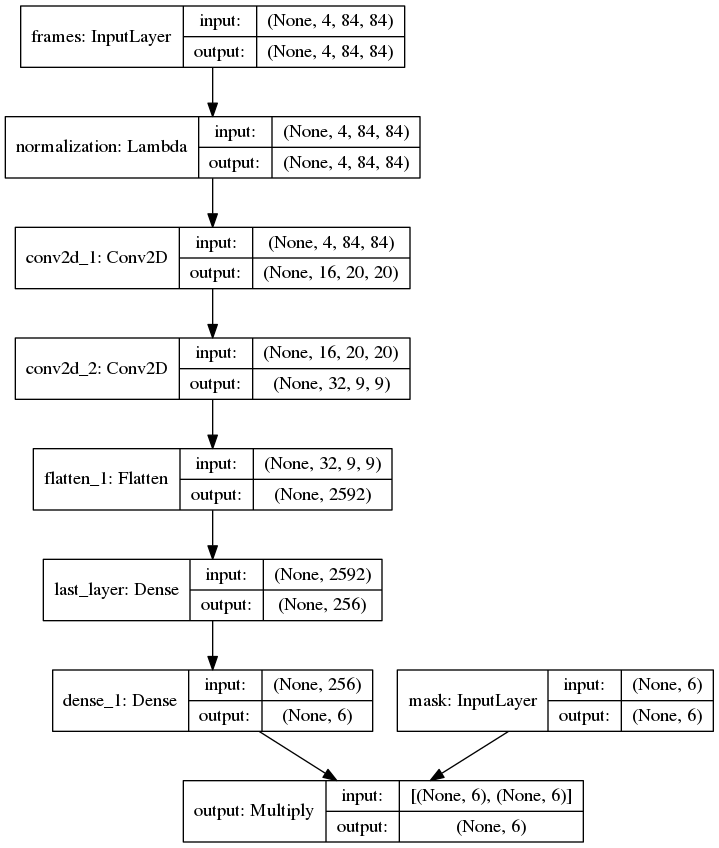
\includegraphics[width=\linewidth]{model.png}
	\captionof{figure}{DQN architecture}
	\end{subfigure}
	%
	\begin{subfigure}[b]{0.59\textwidth}
	\centering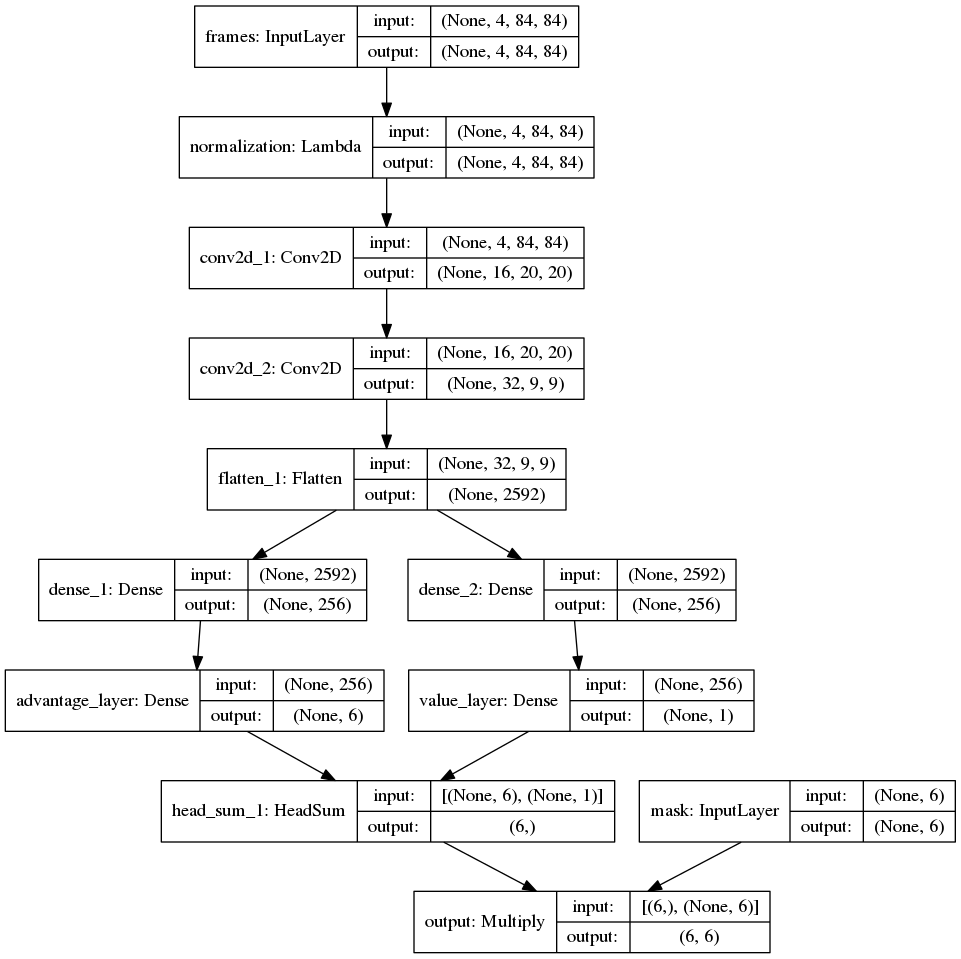
\includegraphics[width=\linewidth]{duel.png}
	\captionof{figure}{Duel DQN architecture}
	\end{subfigure}
	\setcounter{figure}{0}    
	\captionof{figure}{Architecture implemented in this project}
\end{figure*}
\begin{figure*}
	\centering
	\begin{subfigure}{0.49\textwidth}
		\begin{minipage}{\linewidth}
			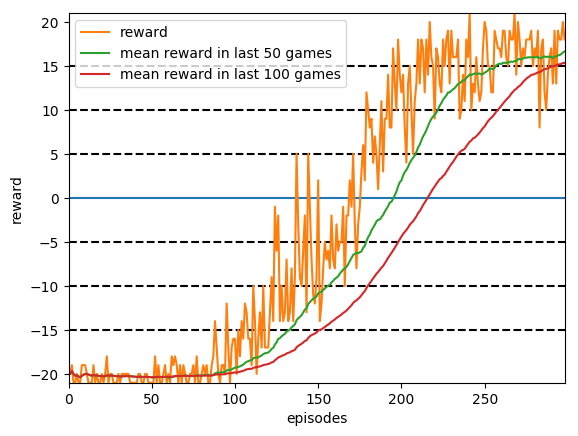
\includegraphics[width=\linewidth]{DDQN_reward.png}
		\end{minipage}\vfill
		\begin{minipage}{\linewidth}
			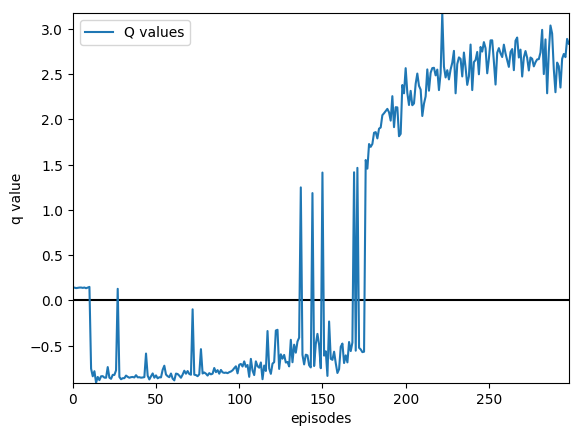
\includegraphics[width=\linewidth]{DDQN_qval.png}
		\end{minipage}\vfill
		\begin{minipage}{\linewidth}
			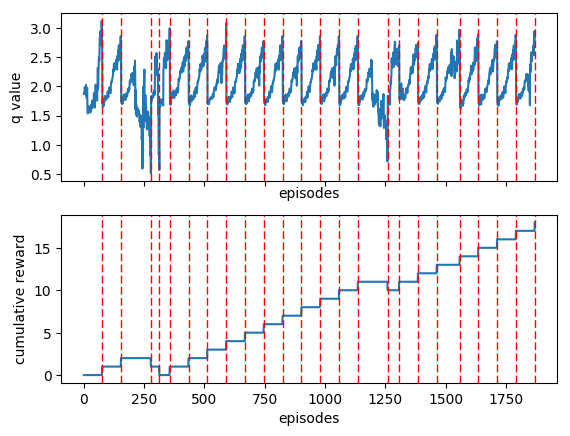
\includegraphics[width=\linewidth]{DDQN_game.png}
		\end{minipage}\vfill
		\caption{DQN with target network results}
	\end{subfigure}
		\begin{subfigure}{0.49\textwidth}
			\centering
			\begin{minipage}{\linewidth}
				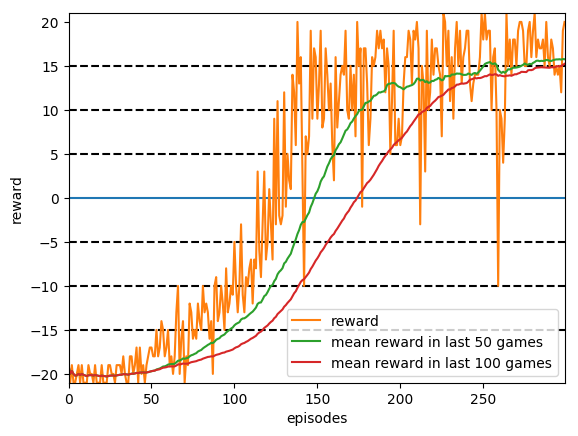
\includegraphics[width=\linewidth]{duel_DDQN_reward.png}
			\end{minipage}\vfill
			\begin{minipage}{\linewidth}
				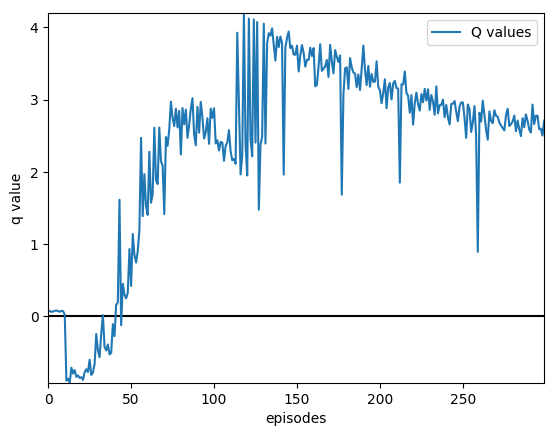
\includegraphics[width=\linewidth]{duel_DDQN_qval.png}
			\end{minipage}\vfill
			\begin{minipage}{\linewidth}
				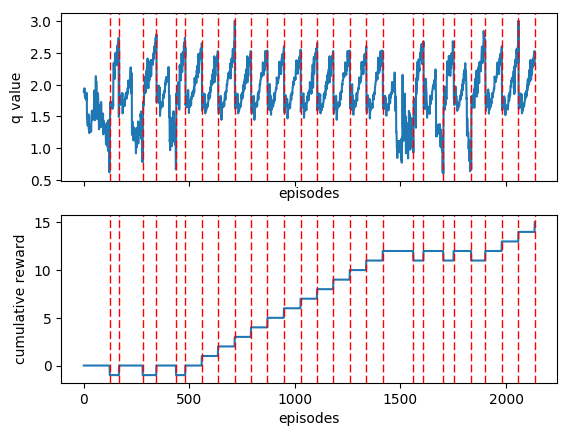
\includegraphics[width=\linewidth]{duel_DDQN_game.png}
			\end{minipage}	\vfill
			\caption{duel DQN with target network results}
		\end{subfigure}
	\setcounter{figure}{1}    
	\captionof{figure}{Experiments using simple memory buffer}
\end{figure*}
\begin{figure*}
	\centering
	\begin{subfigure}{0.49\textwidth}
		\begin{minipage}{\linewidth}
			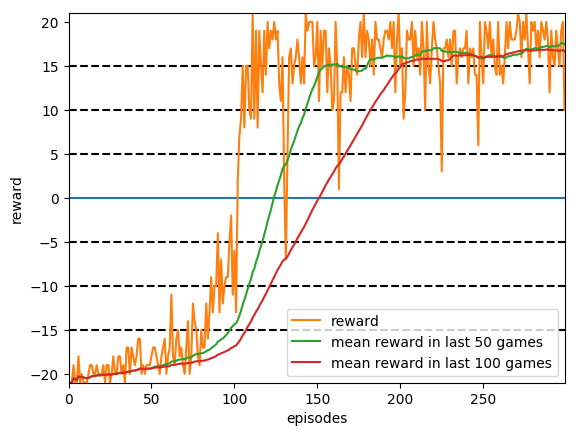
\includegraphics[width=\linewidth]{prior_DDQN_reward.png}
		\end{minipage}\vfill
		\begin{minipage}{\linewidth}
			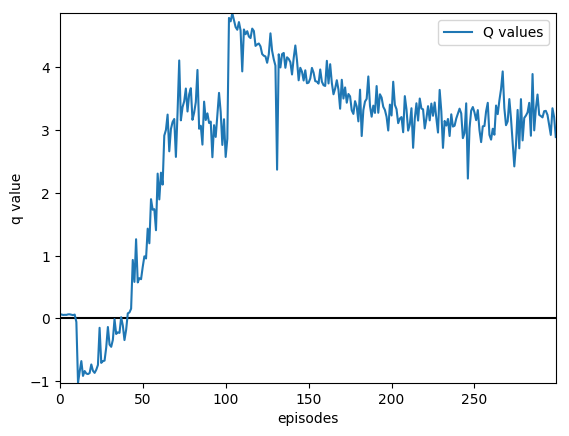
\includegraphics[width=\linewidth]{prior_DDQN_qval.png}
		\end{minipage}\vfill
		\begin{minipage}{\linewidth}
			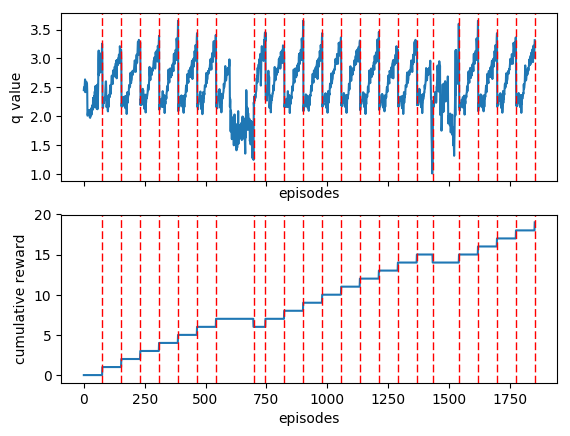
\includegraphics[width=\linewidth]{prior_DDQN_game.png}
		\end{minipage}\vfill
		\caption{DQN with target network results}
	\end{subfigure}
	\begin{subfigure}{0.49\textwidth}
		\centering
		\begin{minipage}{\linewidth}
			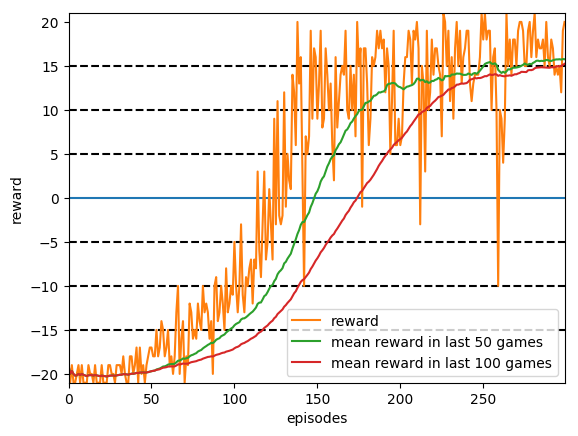
\includegraphics[width=\linewidth]{duel_DDQN_reward.png}
		\end{minipage}\vfill
		\begin{minipage}{\linewidth}
			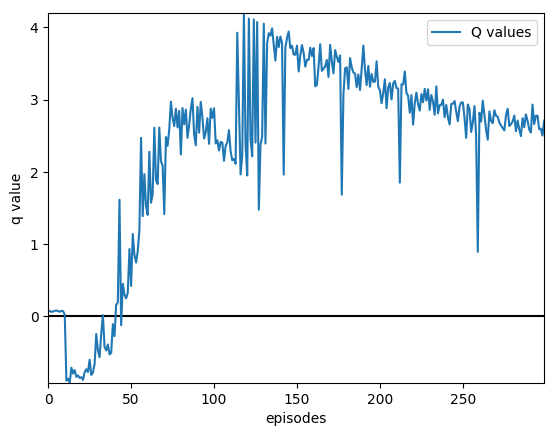
\includegraphics[width=\linewidth]{duel_DDQN_qval.png}
		\end{minipage}\vfill
		\begin{minipage}{\linewidth}
			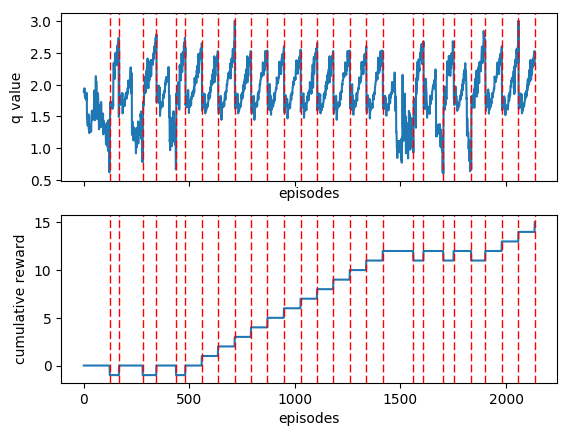
\includegraphics[width=\linewidth]{duel_DDQN_game.png}
		\end{minipage}	\vfill
		\caption{duel DQN with target network results}
	\end{subfigure}
	\setcounter{figure}{2}    
	\captionof{figure}{Experiments using a prioritized memory buffer}
\end{figure*}
\FloatBarrier
\begin{thebibliography}{9}
	
	\bibitem{playAtariGame}
	 Volodymyr Mnih, Koray Kavukcuoglu, David Silver, Alex Graves,
	 Ioannis Antonoglou, Daan Wierstra, and Martin Riedmiller. \textit{Playing
	 atari with deep reinforcement learning}
	
	\bibitem{playAtariGameHuman}
	Volodymyr Mnih, Koray Kavukcuoglu, David Silver, Andrei A Rusu,
	Joel Veness, Marc G Bellemare, Alex Graves, Martin Riedmiller, Andreas
	K Fidjeland, Georg Ostrovski, et al. Human-level control through
	deep reinforcement learning.
	
\end{thebibliography}
\end{document}
